\section{Etherless-Smart}
	
\subsection{Overview}
	Etherless-smart is the module which handles transactions on the Ethereum blockchain. It consists of a set of Ethereum smart contracts that handle the communication between Etherless-cli and Etherless-server as well as the payment of this work using ETH currency.
	
\subsection{Architecture} % Descrizione dell'architettura utilizzata, compresi i design pattern
		Our goals when developing Etherless-smart were upgradeability and extensibility. For these reasons said module consists of three separate smart contracts:
		\begin{itemize}
			\item \textbf{EtherlessSmart:} is the main contract which serves as the middleman between Etherless-cli and Etherless-server. Each one of its methods is either invoked by Etherless-cli to send the requests or by Etherless-server to transmit the responses;
			\item \textbf{EtherlessStorage:} is the storage contract. It stores all relevant information regarding the Javascript functions which can be called when using \textit{Etherless}. Moreover, it contains some utility methods to perform useful operations on this data;
			\item \textbf{EtherlessEscrow:} is the contract which manages everything in regards to monetary transactions. It contains details of every pending transaction and its methods have been implemented to manage an escrow payment.
		\end{itemize}
		
%Descrizione accurata dei metodi presenti nel modulo
\subsubsection{EtherlessSmart}
	\begin{figure}[H]
		\centering
		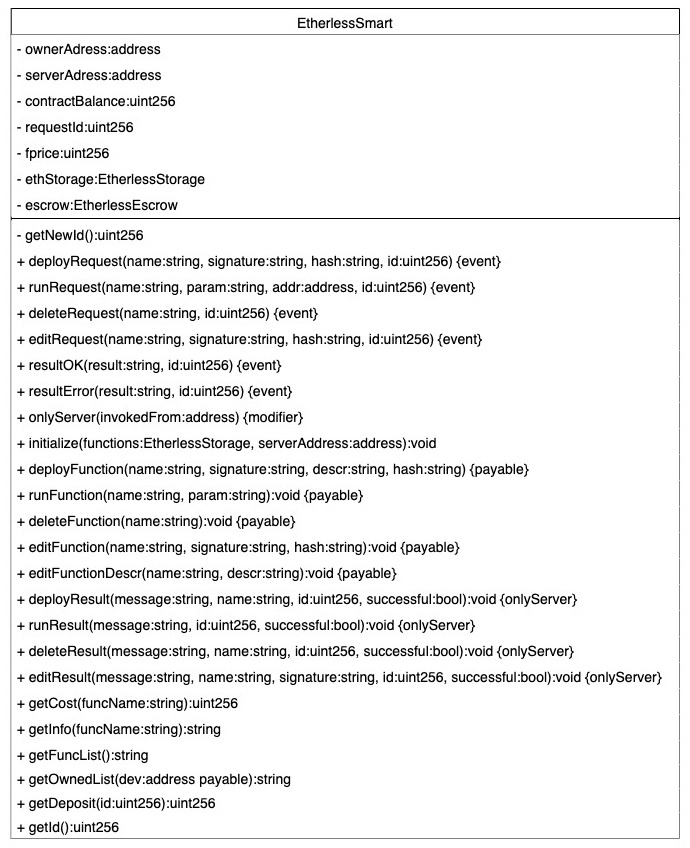
\includegraphics[width=0.6\linewidth]{diagrammi/etherless-smart/EtherlessSmart.jpg}
		\caption{Class diagram of EtherlessSmart}
	\end{figure}

\subsubsubsection*{Attributes}
	\begin{itemize}
		\item \textbf{ownerAddress:} 
		\item \textbf{contractBalance:}
		\item \textbf{requestId:}
		\item \textbf{ethStorage:}
		\item \textbf{escrow:}
	\end{itemize}
\subsubsubsection*{Modifiers}
	\begin{itemize}
		\item \textbf{onlyServer}
	\end{itemize}
\subsubsubsection*{Events}
	\begin{itemize}
		\item \textbf{runRequest}
		\item \textbf{deployRequest}
		\item \textbf{editRequest}
		\item \textbf{deleteRequest}
		\item \textbf{resultOK}
		\item \textbf{resultError}
	\end{itemize}
\subsubsubsection*{Methods}
	\begin{itemize}
		\item \textbf{deployFunction:}
		\item \textbf{runFunction:}
		\item \textbf{editFunction:}
		\item \textbf{deleteFunction:}
		\item \textbf{deployResult:}
		\item \textbf{runResult:}
		\item \textbf{editResult:}
		\item \textbf{deleteResult:}
		\item \textbf{getCost:}
		\item \textbf{getInfo:}
		\item \textbf{getFuncList:}
		\item \textbf{getNewId:}
	\end{itemize}
		
\subsubsection{EtherlessStorage}
	\begin{figure}[H]
		\centering
		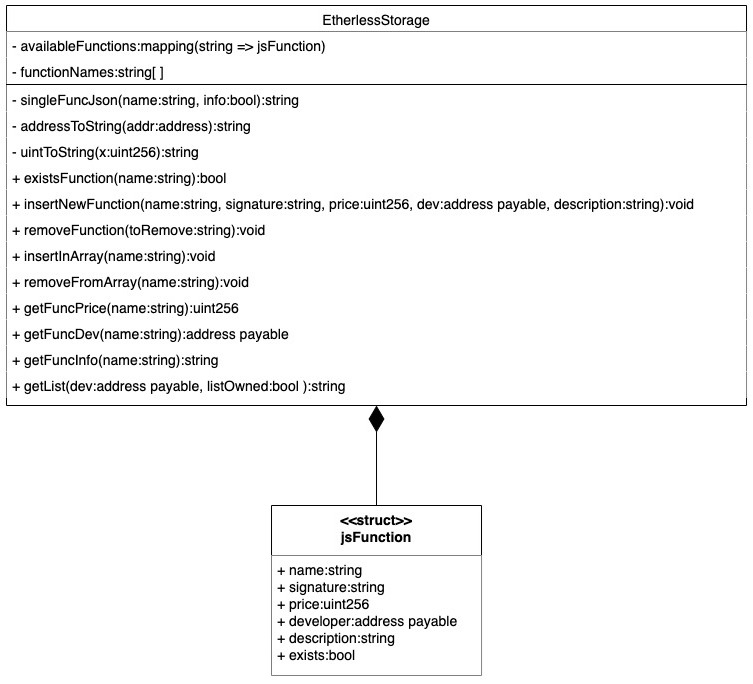
\includegraphics[width=0.6\linewidth]{diagrammi/etherless-smart/EtherlessStorage.jpg}
		\caption{Class diagram of EtherlessStorage}
	\end{figure}

\subsubsubsection*{Attributes}
	\begin{itemize}
		\item \textbf{availableFunctions:} mapping that stores details regarding all functions that have been deployed. Each entry is a key-value pair where the key is the name of the function and the value is a \texttt{jsFunction} struct;
		\item \textbf{functionNames:} array containing the names of all functions that have been deployed. The existence of this array is required since the key value of the \texttt{availableFunctions} mapping cannot be used to perform logical operations;
	\end{itemize}
\subsubsubsection*{Methods}
	\begin{itemize}
		\item \textbf{singleFuncJson:} converts the content of a \texttt{jsFunction} struct into a string written in JSON format;
		\item \textbf{addressToString:} converts an address to a string;
		\item \textbf{uintToString:} converts an unsigned integer to a string;
		\item \textbf{existsFunction:} checks if a function is in \texttt{availableFunctions};
		\item \textbf{insertNewFunction:} adds a function to the \texttt{availableFunctions} mapping;
		\item \textbf{removeFunction:} removes a function from the \texttt{availableFunctions} mapping;
		\item \textbf{insertInArray:} adds a function to the \texttt{functionNames} array;
		\item \textbf{removeFromArray:} removes a function from the \texttt{functionNames} array;
		\item \textbf{getFuncPrice:} returns the price of execution of a certain function;
		\item \textbf{getFuncDev:} returns the developer address of a certain function;
		\item \textbf{getList:} returns the name of all functions a user can execute when using \textit{Etherless};
		\item \textbf{getFuncInfo:} returns all information regarding a function;
		\item \textbf{compareString:} compares two strings using a reasonable gas amount;
	\end{itemize}
		
\subsubsection{EtherlessEscrow}
	\begin{figure}[H]
		\centering
		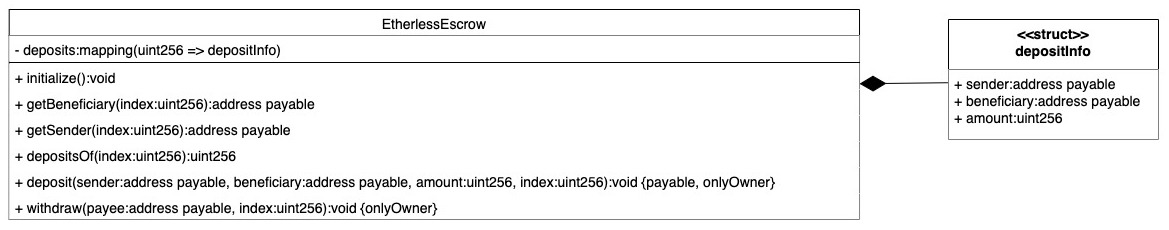
\includegraphics[width=1\linewidth]{diagrammi/etherless-smart/EtherlessEscrow.jpg}
		\caption{Class diagram of EtherlessEscrow}
	\end{figure}

\subsubsubsection*{Attributes}
	\begin{itemize}
		\item \textbf{deposits:} mapping that stores details regarding all pending transaction. Each entry is a key-value pair where the key is a unique identifier and the value is a \texttt{depositInfo} struct;	
		\end{itemize}
\subsubsubsection*{Methods}
	\begin{itemize}
		\item \textbf{getBeneficiary:} returns the beneficiary of the transaction from the \texttt{deposits} mapping having the key \texttt{index};
		\item \textbf{getSender:} returns the sender of the transaction from the \texttt{deposits} mapping having the key \texttt{index};
		\item \textbf{depositsOf:} returns the amount deposited in \texttt{deposits} identified by the key \texttt{index};
		\item \textbf{deposit:} stores the amount sent during a transaction, its sender and its beneficiary in \texttt{deposits} with the key value \texttt{index};
		\item \textbf{withdraw:} withdraws and sends the amount stored in the \texttt{deposits} mapping having the key \texttt{index} to the \texttt{payee} address;
	\end{itemize}

\subsection{UML}
\begin{figure}[H]
		\centering
		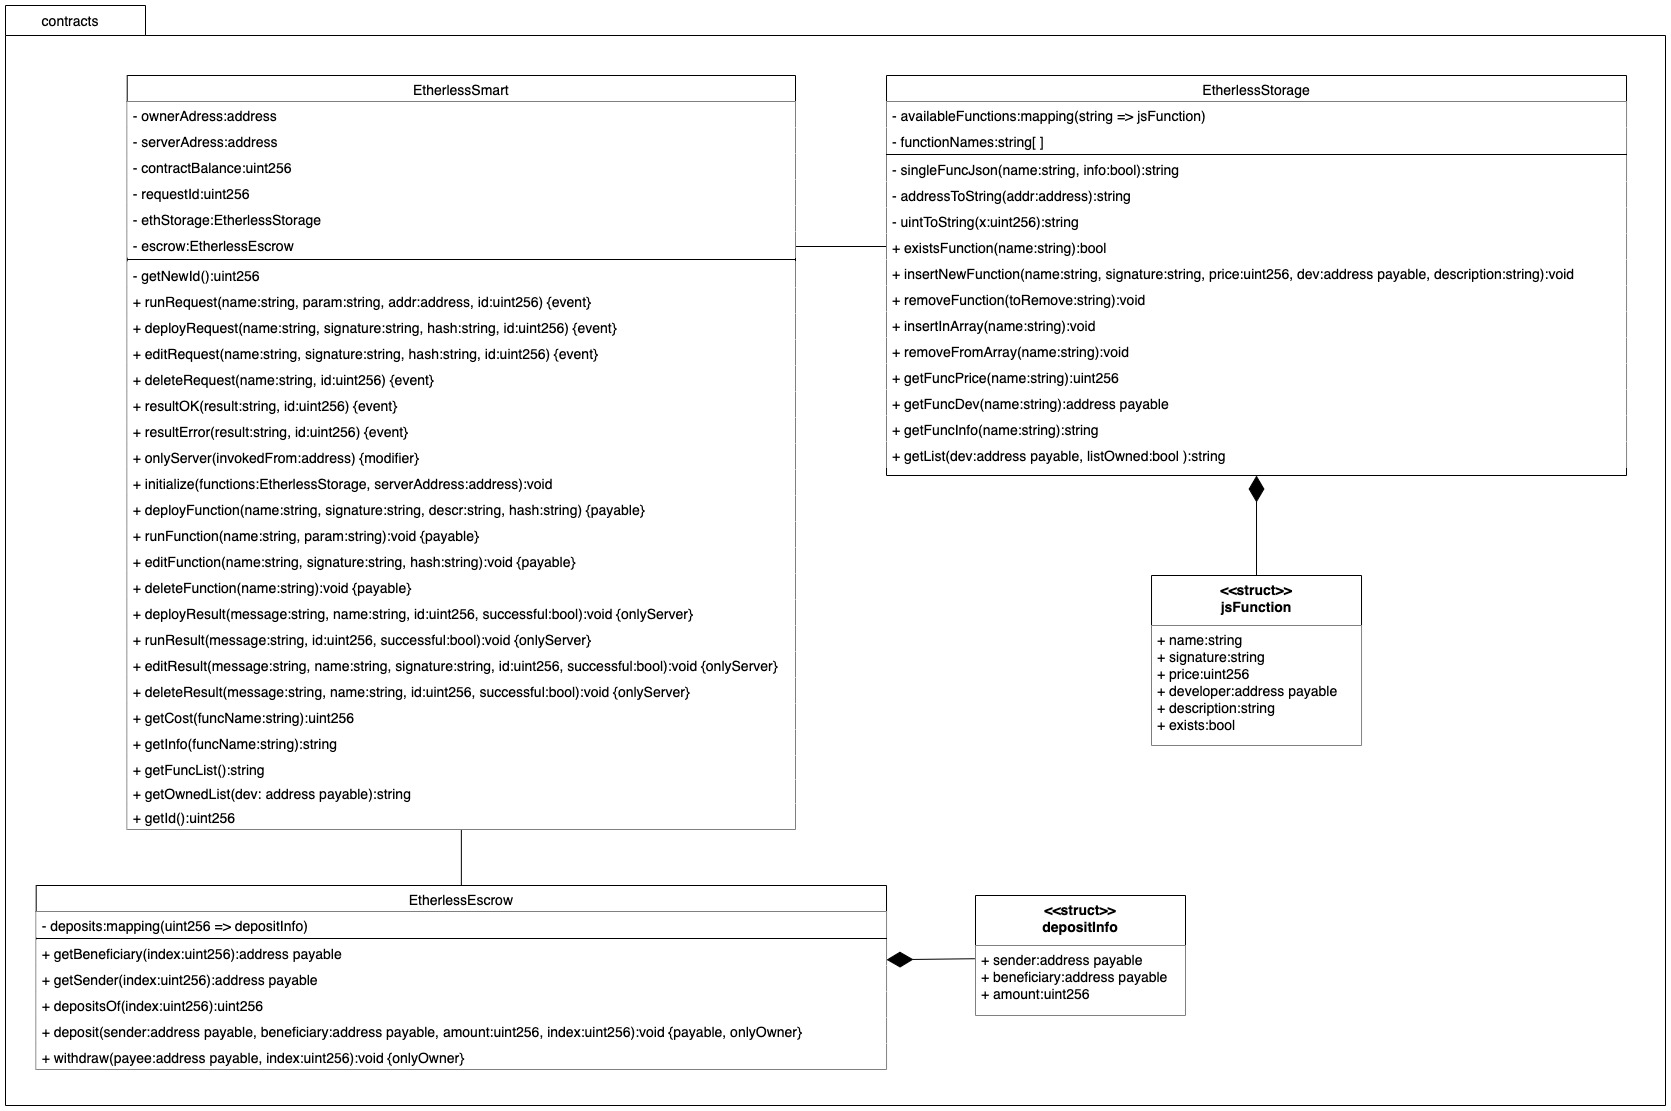
\includegraphics[width=1\linewidth]{diagrammi/etherless-smart/Etherless-smart.jpg}
		\caption{Class diagram of Etherless-smart module}
	\end{figure}
		
\subsection{Extensions}  %Possibili sviluppi futuri